../cictikz/src/cictikz/data/tex/cictikz_preamble.tex

% Battery charging profile, redrawn from the hand-made chart
% (media/charge_graph.png): trickle charge below V_TRICKLE_FAST, then
% constant current at I_CHGLIM while the voltage climbs, constant
% voltage at V_TERM while the current decays, and charging complete
% when it reaches I_TERM. Concept curves, not data: the shapes say
% "flat", "climbs" and "decays", nothing more. Red carries the voltage
% and blue the current, as in the original.

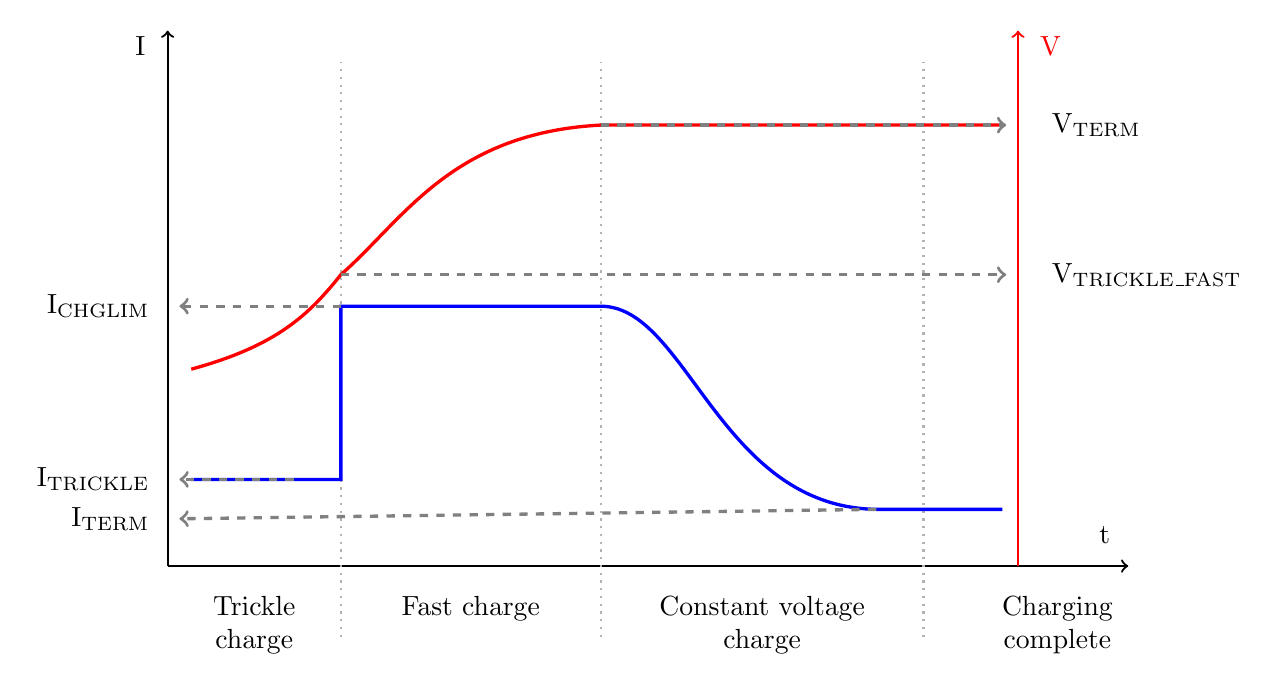
\begin{tikzpicture}[thick]

  % ---- axes ----
  \draw[->] (0,0) -- (0,6.8);
  \node[anchor=east] at (-0.15,6.6) {I};
  \draw[->] (0,0) -- (12.2,0);
  \node[anchor=south east] at (12.1,0.15) {t};
  \draw[red, ->] (10.8,0) -- (10.8,6.8);
  \node[red, anchor=west] at (10.95,6.6) {V};

  % ---- phase boundaries ----
  \foreach \x in {2.2, 5.5, 9.6} {
    \draw[gray!60, dotted] (\x,-0.9) -- (\x,6.4);
  }
  \node[anchor=north, align=center] at (1.1,-0.25) {Trickle\\charge};
  \node[anchor=north] at (3.85,-0.25) {Fast charge};
  \node[anchor=north, align=center] at (7.55,-0.25) {Constant voltage\\charge};
  \node[anchor=north, align=center] at (11.3,-0.25) {Charging\\complete};

  % ---- the current (blue): trickle step, constant current, decay ----
  \draw[blue, very thick] (0.3,1.1) -- (2.2,1.1) -- (2.2,3.3) -- (5.5,3.3)
    .. controls (6.6,3.3) and (7.0,0.75) .. (9.0,0.72)
    -- (10.6,0.72);

  % ---- the voltage (red): slow trickle rise, climb, terminal flat ----
  \draw[red, very thick] (0.3,2.5)
    .. controls (1.4,2.8) and (1.8,3.2) .. (2.2,3.7)
    .. controls (3.0,4.4) and (3.6,5.5) .. (5.5,5.6)
    -- (10.6,5.6);

  % ---- thresholds: grey dashed annotation arrows ----
  \draw[gray, dashed, very thick, ->] (2.2,3.3) -- (0.15,3.3);
  \node[anchor=east] at (-0.1,3.3) {$\mathrm{I_{CHGLIM}}$};
  \draw[gray, dashed, very thick, ->] (1.6,1.1) -- (0.15,1.1);
  \node[anchor=east] at (-0.1,1.1) {$\mathrm{I_{TRICKLE}}$};
  \draw[gray, dashed, very thick, ->] (9.0,0.72) -- (0.15,0.6);
  \node[anchor=east] at (-0.1,0.6) {$\mathrm{I_{TERM}}$};
  \draw[gray, dashed, very thick, ->] (5.5,5.6) -- (10.65,5.6) ;
  \node[anchor=west] at (11.1,5.6) {$\mathrm{V_{TERM}}$};
  \draw[gray, dashed, very thick, ->] (2.2,3.7) -- (10.65,3.7);
  \node[anchor=west] at (11.1,3.7) {$\mathrm{V_{TRICKLE\_FAST}}$};

\end{tikzpicture}
\end{document}
